\section{Diagramme de cas d'utilisation général}
\noindent
La figure ~\ref{fig:recherchearabe} illustre le diagramme de cas d'utilisation gènèral de notre premier sprint, qui est la recherche en Français.

\begin{figure}[H]
	\centering
	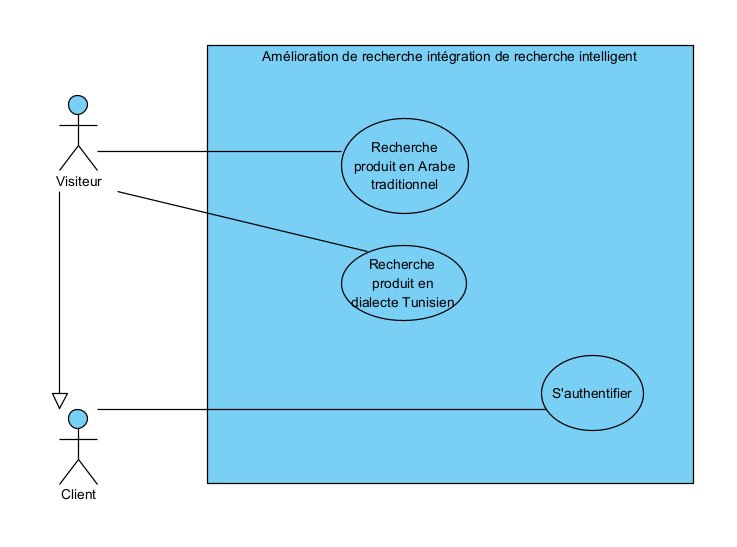
\includegraphics[width=1\textwidth]{logos/cusprint2.png}
	\caption{Diagramme de cas d'utilisation général du Sprint 2}
	\label{fig:recherchearabe}
\end{figure}

\section{Description textuelle des cas d’utilisations}
Une fois les divers cas d'utilisation présentés, nous examinerons de plus près certains
d'entre eux en fournissant la description textuelle de certains d'entre eux.

\newpage
\subsection{Description textuelle du CU « Rechercher produit en Arabe traditionnel »}
\noindent
\textbf{Titre:} Rechercher produit en Arabe traditionnel \\
\textbf{Résumé:} Le client saisit son terme de recherche en Arabe traditionnel, en cliquant sur la boutton pour rechercher le(s) produit(s) qu'il veut chercher. \\
\textbf{Acteur Principal:} Client \\
\textbf{Précondition:} \begin{enumerate}
	\item Le client (ou le visiteur) sont sur la page de recherche
	\item Le client (ou le visiteur) a saisi son terme de recherche en Arabe traditionnel
	\item Le client (ou le visiteur) a cliqué sur "Rechercher"
\end{enumerate}
\textbf{Postcondition:} Le(s) produit(s) que le client cherche est renvoyé, si'il n'existe pas, le systéme renvoie des produits similaires comme suggestion. \\
\textbf{Scénario de base: }
\begin{enumerate}
	\item Le client saisit son terme de recherche.
	\item Le client clique sur la boutton "Rechercher"
	\item Le système prend la terme de recherche, en vérifiant que c'est en Arabe traditionnel, et le traduit en Français.
	\item Le systéme prend cette terme de recherche, et performe les étapes nécessaires pour la convertir en vecteur.
	\item Le systéme compare cette vecteur contre les vecteurs dans Elasticsearch.
	\item Le systéme renvoie les produits.
\end{enumerate}

\newpage
\textbf{Scénario alternatifs : }
\begin{enumerate}
	\item La terme de recherche est vide:
	      \begin{enumerate}
		      \item Le système affiche un message d'erreur informant le client que la terme de recherche est requis.
		      \item Retour à l'étape 1 du scénario de base.
	      \end{enumerate}
	\item La terme de recherche n'est pas en Arabe traditionnel:
	      \begin{enumerate}
		      \item Le système suppose que le terme recherché est en Français.
		      \item Passer à la 4ème étape des scénarios de base.
	      \end{enumerate}
	\item Le(s) produit(s) que le client cherche n'existe pas.
	      \begin{enumerate}
		      \item Le systéme essaie de renvoyer les produits les plus similaires comme des suggestions.
		      \item Retour à l'étape 1 du scénario de base.
	      \end{enumerate}
\end{enumerate}


\subsection{Description textuelle du CU « Rechercher produit en Arabe en dialecte Tunisien »}
\noindent
\textbf{Titre:} Rechercher produit en Arabe en dialecte Tunisien \\
\textbf{Résumé:} Le client saisit son terme de recherche en Arabe en dialecte Tunisien, en cliquant sur la boutton pour rechercher le(s) produit(s) qu'il veut chercher. \\
\textbf{Acteur Principal:} Client \\
\textbf{Précondition:} \begin{enumerate}
	\item Le client (ou le visiteur) son sur la page de recherche
	\item Le client (ou le visiteur) a saisi son terme de recherche en Arabe en dialecte Tunisien
	\item Le client (ou le visiteur) a cliqué sur "Rechercher"
\end{enumerate}
\textbf{Postcondition:} Le(s) produit(s) que le client cherche est renvoyé, si'il n'existe pas, le systéme renvoie des produits similaires comme suggestion. \\
\textbf{Scénario de base: }
\begin{enumerate}
	\item Le client saisit son terme de recherche en Arabe en dialecte Tunisien.
	\item Le client clique sur la boutton "Rechercher"
	\item Le système prend la terme de recherche, en vérifiant que c'est en Arabe en dialecte Tunisien, et le traduit en Français.
	\item Le systéme prend cette terme de recherche, et performe les étapes nécessaires pour la convertir en vecteur.
	\item Le systéme compare cette vecteur contre les vecteurs dans Elasticsearch.
	\item Le systéme renvoie les produits.
\end{enumerate}

\textbf{Scénario alternatifs : }
\begin{enumerate}
	\item La terme de recherche est vide:
	      \begin{enumerate}
		      \item Le système affiche un message d'erreur informant le client que la terme de recherche est requis.
		      \item Retour à l'étape 1 du scénario de base.
	      \end{enumerate}
	\item La terme de recherche n'est pas en Arabe en dialecte Tunisien:
	      \begin{enumerate}
		      \item Le système suppose que le terme recherché est en Français.
		      \item Passer à la 4ème étape des scénarios de base.
	      \end{enumerate}

	\item Le(s) produit(s) que le client cherche n'existe pas.
	      \begin{enumerate}
		      \item Le systéme essaie de renvoyer les produits les plus similaires comme des suggestions.
		      \item Retour à l'étape 1 du scénario de base.
	      \end{enumerate}
\end{enumerate}